\chapter{Các thí nghiệm tính toán}
Trong phần này, chúng ta sẽ mô tả các thí nghiệm tính toán. Trước tiên, chúng tôi giới thiệu một tập hợp những sự điều chỉnh cấu hình trong Phần 4.1. Trong Phần 4.2, chúng tôi đánh giá hiệu suất của các kiến trúc heuristic được đề xuất trên những sự điều chỉnh cấu hình. Trong Phần 4.3, chúng tôi mô tả cách điều chỉnh các tham số của ALNS heuristic và trong Phần 4.4, chúng tôi trình bày các kết quả thu được từ ALNS heuristic và ALNS heuristic đơn giản hơn.

\section{Điều chỉnh cấu hình}
Đầu tiên, xác định một tập hợp các trường hợp điều chỉnh cấu hình đại diện. Các trường hợp điều chỉnh phải có kích thước khá hạn chế vì chúng tôi muốn thực hiện nhiều thử nghiệm về các vấn đề cần điều chỉnh và bằng cách nào đó chúng phải liên quan đến các vấn đề mà phỏng đoán của chúng tôi đang nhắm tới. Trong trường hợp hiện tại, chúng tôi muốn giải quyết một số cấu hình điểm chuẩn tiêu chuẩn (standard benchmark instances) và một tập hợp các cấu hình mới được tạo ngẫu nhiên.
Bộ điều chỉnh của chúng tôi bao gồm 16 trường hợp. Bốn trường hợp đầu tiên là $LR1\_2\_1$, $LR202$, $LRC1\_2\_3$ và $LRC204$ từ bài toán điểm chuẩn của Li và Lim (2001), chứa từ 50 đến 100 yêu cầu. Số lượng phương tiện khả dụng đã được đặt nhiều hơn một so với số lượng mà Li và Lim đã báo cáo để giúp những phỏng đoán dễ dàng tìm ra giải pháp mà không cần yêu cầu trong ngân hàng yêu cầu. 12 phiên bản cuối cùng là các phiên bản được tạo ngẫu nhiên. Các trường hợp này bao gồm cả các vấn đề về một kho và nhiều kho và các vấn đề với các yêu cầu chỉ có thể được phục vụ bởi một tập hợp con của đội xe. Tất cả các vấn đề được tạo ngẫu nhiên chứa 50 yêu cầu.

\section{Đánh giá kiến trúc heuristic}
Đầu tiên, chúng tôi kiểm tra xem các kiến trúc heuristic đơn giản từ Phần 3.2 thực hiện như thế nào đối với các vấn đề điều chỉnh, để xem chúng hoạt động tốt đến mức nào khi không có khung LNS. Các kiến trúc heuristic regret-1, regret-2, regret-3, regret-4 và regret-m đã được triển khai. Bảng 2 trình bày kết quả của thử nghiệm. Vì các kiến trúc heuristic mang tính xác định, các kết quả được tạo ra bằng cách áp dụng các phỏng đoán cho từng vấn đề trong số 16 vấn đề được thử nghiệm.

\begin{table}
    \caption{Performance of Construction Heuristics}
    \begin{tabular}{c c c c c c} 
        \hline 
        & Basic greedy & Regret-2 & Regret-3 & Regret-4 & Regret-m\\ [0.5ex] 
        \hline 
        Avg.gap (\%) & 40.7 & 30.3 & 26.3 & 26.0 & 27.7 \\ 
        Fails & 3 & 3 & 3 & 2 & 0 \\
        Time (s) & 0.02 & 0.02 & 0.02 & 0.02 & 0.03 \\ [1ex] 
        \hline 
    \end{tabular}
    \\ [1ex] 
    \caption{ \textit{Ghi chú: Mỗi cột trong bảng tương ứng với một trong các contruction heuristic. Những kinh nghiệm đơn giản này không phải lúc nào cũng có thể xây dựng một giải pháp trong đó tất cả các yêu cầu đều được đáp ứng; do đó, đối với mỗi heuristic, chúng tôi báo cáo số lần mà điều này xảy ra trong hàng "lỗi". Hàng Avg.gap hiển thị sự khác biệt tương đối trung bình giữa giải pháp được tìm thấy và giải pháp được biết đến nhiều nhất. Chỉ những giải pháp mà tất cả các yêu cầu đều được đáp ứng mới được đưa vào tính toán Avg.gap. Hàng cuối cùng hiển thị thời gian trung bình (tính bằng giây) cần thiết để áp dụng heuristic cho một vấn đề, chạy trên Pentium IV 1.5 GHz.}}
\end{table}

Kết quả cho thấy các kiến trúc heuristic được đề xuất rất nhanh nhưng cũng rất không chính xác. Thuật toán tham lam cơ bản có phỏng đoán tồi tệ nhất, trong khi tất cả các regret heuristics đều có thể so sánh được với giải pháp chất lượng. Tuy nhiên, regret-m lại nổi bật lên vì nó có thể đáp ứng mọi yêu cầu trong mọi vấn đề. Có lẽ có thể cải thiện các kết quả thể hiện trong Bảng 2 bằng cách đưa ra các yêu cầu hạt giống (seed requests) như đề xuất của Solomon (1987). Tuy nhiên, chúng tôi sẽ không báo cáo về các thí nghiệm như vậy trong bài báo này. Có thể khá bất ngờ khi những phỏng đoán rất không chính xác này có thể được sử dụng làm nền tảng cho một phỏng đoán tìm kiếm cục bộ chính xác hơn nhiều, nhưng như chúng ta sẽ thấy trong các phần sau rằng điều này thực sự có thể xảy ra.


\section{Điều chỉnh tham số}
Phần này của bài viết phục vụ hai mục đích. Đầu tiên là mô tả cách tìm thấy các tham số được sử dụng để tạo ra kết quả trong Phần 4.4. Tiếp theo, trình bày phần nào của phỏng đoán đóng góp nhiều nhất vào chất lượng giải pháp.

\subsection{Các tham số}
Phần này xác định các tham số cần được điều chỉnh. Đầu tiên chúng tôi xem xét các tham số loại bỏ. Shaw removal được kiểm soát bởi năm tham số: $\varphi, \chi, \psi, \omega$, và $p$, trong khi "worst removal" được kiểm soát bởi một tham số $p_{worst}$. Sự loại bỏ ngẫu nhiên sẽ không có tham số. Các heuristics thêm là tham số tự do khi chúng tôi đã chọn mức độ regret.
Để kiểm soát các tiêu chí được chấp nhận, chúng tôi sử dụng hai tham số, $w$ và $c$. Thuật toán điều chỉnh trọng số được kiểm soát bởi bốn tham số: $\sigma_1$, $\sigma_2$, $\sigma_3$ và $r$. Cuối cùng, chúng ta phải xác định độ nhiễu $\eta$ và a tham số $\zeta$ có tác dụng kiểm soát số lượng yêu cầu bị loại bỏ trong mỗi lần lặp. Trong mỗi lần lặp lại, chúng tôi đã chọn một số ngẫu nhiên $p$ thỏa mãn $4 \leq p \leq min(100, \zeta n)$, và xóa $p$ yêu cầu. Việc tìm kiếm được dừng lại sau 25.000 lần lặp LNS vì điều này dẫn đến sự đánh đổi hợp lý giữa thời gian và chất lượng.

\subsection{Điều chỉnh tham số LNS}
Mặc dù một lượng lớn tham số được sử dụng trong ALNS heuristic, nhưng việc tìm ra một tập hợp các tham số hoạt động tốt cho một loạt các vấn đề lại tương đối dễ dàng. Chúng tôi sử dụng chiến lược sau để điều chỉnh các tham số: Đầu tiên, một bộ tham số hợp lý được tạo ra bởi giai đoạn thử và sai đặc biệt; bộ tham số này đã được tìm thấy trong khi phát triển phỏng đoán. Bộ tham số này được cải thiện trong giai đoạn thứ hai bằng cách cho phép một tham số nhận một số giá trị, trong khi các tham số còn lại được giữ cố định. Đối với mỗi bộ tham số, chúng tôi áp dụng phỏng đoán cho tập hợp các vấn đề cần kiểm tra của mình năm lần và hành vi trung bình tốt nhất sẽ được chọn (so sánh về độ lệch trung bình so với các giải pháp tốt nhất đã biết). Sau đó chúng tôi chuyển đến tham số tiếp theo, sử dụng các giá trị được tìm thấy và các giá tri từ tham số điều chỉnh ban đầu cho các tham số chưa được xem xét. Quá trình này tiếp tục cho đến khi tất cả các tham số đã được điều chỉnh. Mặc dù có thể sử dụng lại các tham số bằng cách sử dụng bộ tham số mới làm điểm bắt đầu để tối ưu hóa hơn nữa các tham số, nhưng chúng tôi đã dừng lại sau một lượt.

Một trong những thử nghiệm được thực hiện trong quá trình điều chỉnh tham số nhằm xác định giá trị của tham số $\zeta$, điều này kiểm soát số lượng yêu cầu được loại bỏ trong mỗi lần lặp. Thông số này về mặt trực giác sẽ có tác động đáng kể đến các kết quả mà phương pháp phỏng đoán của chúng ta có thể tạo ra. Chúng tôi đã thử nghiệm phỏng đoán với $\zeta$ nằm trong phạm vi từ 0.05 đến 0.5 với độ dài bước là 0.05. Bảng 3 cho thấy ảnh hưởng của $\zeta$.  Khi $\zeta$ quá thấp, phỏng đoán sẽ không thể đi xa trong mỗi lần lặp và sẽ có nhiều khả năng bị mắc kẹt trong một khu vực dưới mức tối ưu của không gian tìm kiếm. Mặt khác, nếu $\zeta$ lớn, thì chúng ta có thể dễ dàng di chuyển trong không gian tìm kiếm, nhưng chúng ta cũng đang mở rộng khả năng của phương pháp phỏng đoán chèn của mình. Các phỏng đoán chèn hoạt động khá tốt khi chúng phải chèn một số lượng yêu cầu hạn chế vào một phần giải pháp, nhưng chúng không thể xây dựng một giải pháp tốt từ đầu, như đã thấy trong Phần 4.2. Kết quả ở bảng 3 cho thấy theta = 04 là một lựa chọn tốt. Cần lưu ý rằng phỏng đoán sẽ chậm hơn khi tăng theta vì việc xóa và chèn mất nhiều thời gian hơn khi có nhiều yêu cầu hơn; do đó, sự so sánh trong Bảng 3 là không hoàn toàn công bằng.


\begin{table}
    \caption[]{Parameter $\zeta$ vs. Solution Quality}
    %\centering
    \begin{tabular}{c c c c c c c c c c c} 
        \hline
        $\zeta$ & 0.05 & 0.1 & 0.15 & 0.2 & 0.25 & 0.3 & 0.35 & 0.4 & 0.45 & 0.5 \\
        Avg.gap (\%) & 1.75 & 1.65 & 1.21 & 0.97 & 0.81 & 0.71 & 0.81 & 0.49 & 0.57 & 0.57 \\ [1ex]
        \hline 
    \end{tabular}
    \\ [1ex]
    \caption*{ \textit{Ghi chú: Hàng đầu tiên hiển thị Các giá trị Của tham số $\zeta$ đã được kiểm tra và hàng thứ hai hiển thị khoảng cáCh giữa giải pháp trung bình thu được và giải pháp tốt nhất được tạo ra trong thử nghiệm.}}   
\end{table}

Việc điều chỉnh tham số hoàn chỉnh dẫn đến vectơ tham số sau:

($\varphi, \chi, \psi, \omega, p,  p_{worst}, w, c, \sigma_1, \sigma_2, \sigma_3, r, \eta, \zeta$) = (9, 3, 2, 5, 6, 3, 0.05, 0.99975, 33, 9, 13, 0.1, 0.025, 0.4). Các thử nghiệm của chúng tôi cũng chỉ ra rằng có thể cải thiện hiệu suất của thuật toán giảm số phương tiện bằng cách đặt ($w,c$)  = (0.35, 0.9999), trong khi tìm kiếm các giải pháp đáp ứng mọi yêu cầu . Điều này tương ứng với nhiệt độ bắt đầu cao hơn và tốc độ làm mát chậm hơn. Điều này cho thấy rằng cần phải đa dạng hóa hơn khi cố gắng giảm thiểu số lượng phương tiện, so với tình huống mà người ta chỉ giảm thiểu khoảng cách di chuyển.

Để điều chỉnh các tham số, chúng tôi bắt đầu từ dự đoán ban đầu, sau đó điều chỉnh từng tham số một. Khi tất cả các tham số được điều chỉnh, quá trình này sẽ được lặp lại. Bằng cách này, thứ tự hiệu chuẩn đóng một vai trò nhỏ. Mặc dù việc điều chỉnh thông số khá tốn thời gian, nhưng nó có thể dễ dàng được tự động hóa. Trong các bài báo tiếp theo của chúng tôi (Ropke và Pisinger 2006; Pisinger và Ropke 2005), 11 biến thể của bài toán định tuyến phương tiện được giải quyết bằng cách sử dụng phương pháp heuristic được đề xuất trong bài báo này, chúng tôi chỉ điều chỉnh lại một số tham số và thu được kết quả rất thuyết phục. Có vẻ như việc điều chỉnh hoàn toàn các tham số chỉ cần được thực hiện một lần.

\subsection{Cấu hình LNS}
Phần này đánh giá cách thức hoạt động của các phương pháp phỏng đoán loại bỏ và chèn khác nhau khi được sử dụng trong phương pháp ALNS heuristic. Trong hầu hết các trường hợp thử nghiệm, một phương pháp ALNS heuristic đơn giản đã được sử dụng chỉ liên quan đến một phương pháp phỏng đoán loại bỏ và một phương pháp phỏng đoán chèn. Bảng 4 cho thấy một bản tóm tắt của thí nghiệm này.

\begin{center}
    \begin{figure}[]
    \caption{So sánh LNS Heuristics đơn giản và LNS thích ứng đầy đủ với trọng số động}        
    \begin{center}
     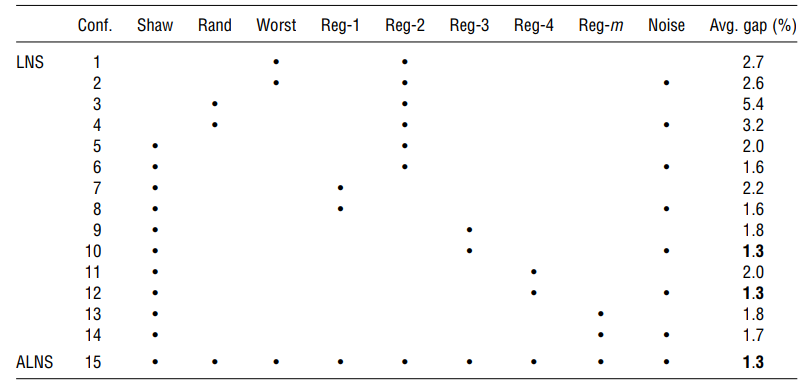
\includegraphics[scale=.5]{figures/Thuy_table4}
    \end{center}
  \textit{Ghi Chú. Cột đầu tiên hiển thị liệu Cấu hình phải được coi là LNS hay ALNS heuristic. Cột thứ hai là số cấu hình, cột 3 đến 5 cho biết heuristics xóa nào đã được sử dụng. Các cột từ 6 đến 10 cho biết heuristics thêm nào đã được sử dụng. Cột 11 cho biết liệu "nhiễu" có được thêm vào chức năng mục tiêu trong khi thêm yêu cầu hay không (trong trường hợp này, "nhiễu" đã được thêm vào hàm mục tiêu trong 50\% số lần thêm đối vi cấu hình đơn giản 1–14 trong khi ở Cấu hình 15, số lần thêm "nhiễu" được kiểm soát bằng phương pháp thích nghi (adaptive method)). Cột 12 Cho thấy hiệu suất trung bình của các heuristic khác nhau. Ví dụ: Trong cấu hình 4, chúng tôi đã sử dụng loại bỏ ngẫu nhiên cùng với phương pháp heuristics thêm regret-2 và chúng tôi đã áp dụng nhiễu cho giá trị mục tiêu. Điều này dẫn đến một tập hợp các giải pháp có giá trị mục tiêu trung bình cao hơn 3,2\% so với các giải pháp tốt nhất được tìm thấy trong toàn bộ thử nghiệm.}
    \end{figure}
\end{center}

Sáu thí nghiệm đầu tiên nhằm mục đích xác định ảnh hưởng của phương pháp xóa heuristic. Chúng tôi thấy rằng phương pháp Shaw removal là tốt nhất, phương pháp the worst removal heuristic đứng thứ hai và xóa heuristic ngẫu nhiên cho hiệu suất kém nhất. Điều này làm ta cảm thấy yên tâm vì nó cho thấy rằng hai phương pháp xóa heuristic phức tạp hơn một chút thực sự tốt hơn so với phương pháp xóa heuristic đơn giản nhất. Những kết quả này cũng minh họa rằng phương pháp xóa heuristic có thể có tác động khá lớn đến chất lượng của giải pháp thu được, do đó, việc thử nghiệm với những phương pháp xóa heuristic khác sẽ rất thú vị và có thể mang lại lợi ích.
Tám thí nghiệm tiếp theo cho thấy hiệu suất của phương pháp thêm heuristic. Ở đây, chúng tôi đã chọn Shaw removal làm cách phỏng đoán loại bỏ vì nó được có hiệu suất trong các thử nghiệm trước đó. Trong các thí nghiệm này, chúng ta thấy rằng tất cả các phương pháp thêm heuristic đều hoạt động khá tốt và chúng khá khó phân biệt với nhau. Regret-3 và regret-4 kết hợp với bổ sung nhiễu (noise) tốt hơn một chút so với phần còn lại. Tuy nhiên, khi quan sát tất cả các thí nghiệm, việc áp dụng nhiễu dường như giúp ích cho phỏng đoán. Thật thú vị khi lưu ý rằng phương pháp thêm heuristic cơ bản hoạt động gần giống như phỏng đoán regret khi được sử dụng trong khung LNS. Quan sát này có thể chỉ ra rằng phương pháp LNS tương đối mạnh đối với phương pháp thêm đã được sử dụng.
Hàng cuối cùng của Bảng hiển thị hiệu suất của ALNS. Có thể thấy, nó ngang bằng với hai cách tiếp cận đơn giản tốt nhất, nhưng không tốt hơn, điều này thoạt nghe có vẻ đáng thất vọng. Tuy nhiên, kết quả cho thấy rằng cơ chế thích ứng có thể tìm thấy một tập trọng số hợp lý và giả thuyết của chúng tôi là phương pháp ALNS heuristic mạnh hơn phương pháp ALNS heuristic đơn giản hơn. Nghĩa là, cấu hình đơn giản có thể không tạo ra các giải pháp tốt cho các loại vấn đề khác, trong khi ALNS heuristic tiếp tục hoạt động tốt.
Một trong những mục đích của các thí nghiệm trong Phần 4.4 là để xác nhận hoặc bác bỏ giả thuyết này.

\section{Kết quả}
Phần này cung cấp các thí nghiệm tính toán được tiến hành để kiểm tra hiệu suất của heuristic. Có ba mục tiêu chính cho phần này:
\begin{itemize}
    \item Để so sánh phương pháp ALNS heuristic với phương pháp ALNS heuristic đơn giản chỉ chứa một phương pháp phỏng đoán xóa và một phương pháp phỏng đoán thêm.
    \item Để xác định xem các dặc tính nhất định của vấn đề có ảnh hưởng đến khả năng (A)LNS heuristic tìm ra các giải pháp tốt hay không.
    \item Để so sánh phương pháp ALNS heuristic với phương pháp PDPTW heuristic tiên tiến nhất từ tài liệu.
   
\end{itemize}

Để làm rõ liệu ALNS heuristic có đáng giá so với ALNS heuristic đơn giản hay không, chúng tôi sẽ hiển thị kết quả cho cả ALNS heuristic và ALNS heuristic đơn giản tốt nhất từ bảng 4. Cấu hình 12 được chọn làm đại diện cho ALNS heuristic đơn giản vì nó hoạt động tốt hơn một chút so với cấu hình 10. Trong các phần sau, chúng tôi đề cập đến phương pháp ALNS heuristic đơn giản và đầy đủ là ALNS và LNS tương ứng.
Tất cả các thử nghiệm được thực hiện trên PC Pentium IV 1.5 GHz với bộ nhớ trong 256 MB, chạy Linux. Thuật toán đã triển khai sẽ tính toán thời gian và khoảng cách di chuyển bằng cách sử dụng các số dấu phẩy động có độ chính xác gấp đôi. Tham số được tìm thấy trong Phần 4.3.2 đã được sử dụng trong tất cả các thử nghiệm trừ khi có thông báo khác.

\subsection{Tập dữ liệu}
Vì mô hình được xem xét trong bài viết này khá phức tạp nên khó có thể tìm thấy bất kỳ cấu hình điểm chuẩn (benchmark instances) nào cân nhắc chính xác cùng một mô hình và hàm mục tiêu. Các cấu hình điểm chuẩn gần nhất với mô hình được xem xét trong bài viết này là các trường hợp do Nanry và Barnes (2000) xây dựng và các trường hợp do Li và Lim (2001) xây dựng. Cả hai bộ dữ liệu đều là về vấn đề nhận và giao hàng tại một kho hàng với khung thời gian, xây dựng từ bài toán VRPTW.

\begin{center}
    \begin{figure}[htp]
    \caption{Tóm tắt kết quả thu được từ các trường hợp của Li và Lim}        
    \begin{center}
     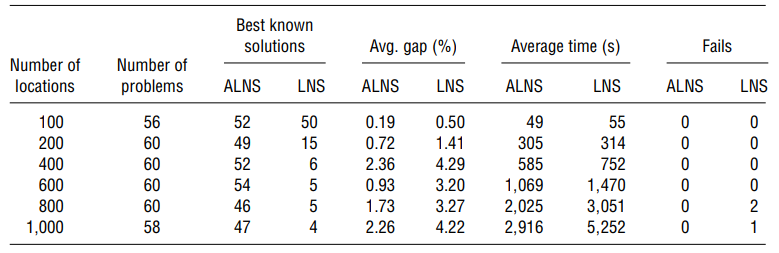
\includegraphics[scale=.5]{figures/Thuy_table5}
    \end{center}
  \textit{Ghi Chú: Cột đầu tiên đưa ra quy mô của vấn đề; cột tiếp theo cho biết số vấn đề trong tập dữ liệu có kích thước cụ thể. Phần còn lại của bảng bao gồm bốn cột chính, mỗi cột được chia thành hai cột con, một cho ALNS và một cho LNS. Cột "Các giải pháp được biết đến nhiều nhất" cho biết có bao nhiêu vấn đề mà giải pháp được biết đến nhiều nhất đã được xác định. Giải pháp được biết đến nhiều nhất là giải pháp được báo cáo bởi Li và Lim hoặc giải pháp tốt nhất được xác định bởi (A)LNS heuristic, tùy thuộc vào giải pháp nào là tốt nhất. Cột tiếp theo cho biết giải pháp trung bình cách giải pháp tốt nhất đã biết bao xa. Con số này được tính trung bình trên tất cả các bài toán có kích thước cụ thể. Cột tiếp theo cho biết thời gian trung bình dành cho heuristic để giải quyết một vấn đề. Cột cuối cùng hiển thị số lần heuristic không tìm ra giải pháp trong đó tất cả các yêu cầu được đáp ứng bởi số lượng phương tiện nhất định trong tất cả các nỗ lực giải quyết một vấn đề cụ thể.}
    \end{figure}
\end{center}

Chúng tôi chỉ báo cáo kết quả trên tập dữ liệu do Li và Lim đề xuất, vì các trường hợp Nanry và Barnes rất dễ giải quyết nhờ kích thước của chúng.
Vấn đề được xem xét bởi Li và Lim đơn giản hơn vấn đề trong bài viết này bởi vì: (1) nó không chứa nhiều kho; (2) tất cả các yêu cầu phải được phục vụ; (3) tất cả các phương tiện được giả định là có thể phục vụ tất cả các yêu cầu. Khi giải quyết các trường hợp của Li và Lim bằng cách sử dụng ALNS heuristic, chúng tôi đặt $\alpha$ bằng 1 và $\beta$ bằng 0 trong hàm mục tiêu của mình. Trong Phần 4.5, chúng tôi coi việc giảm thiểu số lượng phương tiện là ưu tiên hàng đầu trong khi ở Phần 4.4.2, chúng tôi chỉ giảm thiểu độ dài quãng đường cần lái xe.
Để kiểm tra tất cả các khía cạnh của mô hình được đề xuất trong bài báo này, chúng tôi cũng giới thiệu một số trường hợp mới, được tạo ngẫu nhiên. Những trường hợp này được mô tả trong Phần 4.4.3.

\subsection{So sánh ALNS và LNS bằng cách sử dụng các trường hợp của Li Và Lim}
Phần này so sánh ALNS heuristic và LNS heuristic bằng cách sử dụng các cấu hình điểm chuẩn do Li Và Lim (2001) đề xuất. Tập dữ liệu Chứa 354 cấu hình với 100 đến 1,000 vị trí. Có thể tải xuống bộ dữ liệu từ SINTEF.
Trong phần này, chúng tôi sử dụng quãng đường đã đi làm mục tiêu của mình mặc dù giảm thiểu phương tiện là mục tiêu chính cho những trường hợp này. Lý do cho quyết định này là việc giảm thiểu khoảng cách làm cho việc so sánh các phương pháp phỏng đoán trở nên dễ dàng hơn và việc giảm thiểu khoảng cách là mục tiêu ban đầu của phương pháp phỏng đoán được đề xuất. Số lượng phương tiện có sẵn để phục vụ các yêu cầu được đặt thành các giá trị tối thiểu được báo cáo bởi Li Và Lim (2001) trên trang web của họ, rất tiếc là trang này không còn trực tuyến nữa. Các phỏng đoán được áp dụng 10 lần cho mỗi trường hợp với 400 vị trí trở xuống và 5 lần cho từng trường hợp, với hơn 400 địa điểm. Các thí nghiệm được tóm tắt trong bảng 5.
Kết quả cho thấy rằng ALNS heuristic trên cả bốn điều kiện đều hoạt động tốt hơn so với LNS heuristic. Người ta cũng nhận thấy rằng ALNS heuristic thậm chí trở nên hấp dẫn hơn khi kích thước của vấn đề tăng lên. Có vẻ kỳ lạ là LNS heuristic mất nhiều thời gian hơn so với ALNS heuristic khi cả hai đều có cùng một số lần lặp LNS. Lý do cho việc này là Shaw removal heuristic được sử dụng bởi ALNS heuristic tốn nhiều thời gian hơn so với hai phương pháp phỏng đoán xóa khác.

\subsection{Các trường hợp mới}

Phần này cung cấp kết quả về các trường hợp PDPTW được tạo ngẫu nhiên có chứa các đặc điểm của mô hình không được sử dụng trong các bài toán điểm chuẩn của Li Và Lim (2001) được xem xét trong Phần 4.4.2. Các đặc điểm này là: Nhiều kho, các tuyến đường có điểm bắt đầu và điểm kết thúc khác nhau và các yêu cầu đặc biệt chỉ có thể được phục vụ bởi một nhóm phương tiện phụ nhất định. Khi giải các trường hợp này, chúng ta đặt $\alpha$= $\beta$=1 trong hàm mục tiêu sao cho khoảng cách và thời gian được tính trọng số như nhau trong hàm mục tiêu. Chúng tôi không thực hiện giảm thiểu phương tiện vì các phương tiện không đồng nhất. 
Ba loại phân phối địa lý của các yêu cầu được xem xét: Các vấn đề với các vị trí được phân bổ đồng đều trong mặt phẳng, các vấn đề với các vị trí được phân bổ trong 10 cụm và các vấn đề với 50\% các vị trí được đặt trong 10 cụm và 50\% các vị trí được phân bổ đồng đều. Ba loại bài toán này lấy cảm hứng từ các bài toán điểm chuẩn VRPTW của Solomon (1987), và các bài toán tương tự như các bài toán r, c, và RC Solomon tương ứng. Chúng tôi xem xét các vấn đề với 50, 100, 250 và 500 yêu cầu; tất cả đều là vấn đề đa kho. Đối với mỗi kích thước vấn đề chúng tôi tạo ra 12 vấn đề, trong khi chúng tôi thử mọi sự kết hợp của ba đặc điểm được hiển thị bên dưới:
\begin{itemize}
    \item Loại tuyến đường: (1) Tuyến đường bắt đầu và kết thúc tại cùng một vị trí, (2) Tuyến đường bắt đầu và kết thúc ở các vị trí khác nhau.
    nhỏ hơn, có cùng cách giải.
    \item Loại yêu cầu: (1) tất cả các yêu cầu đều là yêu cầu thông thường, (2) 50\% là yêu cầu đặc biệt. Các yêu cầu đặc biệt chỉ có thể được phục vụ bởi một nhóm nhỏ các phương tiện. Trong các vấn đề thử nghiệm, mỗi yêu cầu đặc biệt chỉ có thể được phục vụ bởi 30\% đến 60\% số phương tiện.
    \item Phân phối địa lý: (1) Đồng nhất, (2) Phân cụm Và (3) Bán phân cụm.
\end{itemize}
Có thể tải xuống các phiên bản từ www.diku.dk/ ~sropke. Các phỏng đoán đã được kiểm tra bằng cách áp dụng chúng cho mỗi vấn đề trong số 48 vấn đề 10 lần. Bảng 6 cho thấy một bản tóm tắt các kết quả được tìm thấy. Trong bảng, có thể liệt kê số lượng bài toán mà hai phương pháp heuristics tìm ra lời giải tốt nhất đã biết. Giải pháp tốt nhất đơn giản là giải pháp tốt nhất được tìm thấy trong suốt thí nghiệm này.

\begin{center}
    \begin{figure}[htp]
    \caption{Tóm tắt kết quả thu được từ các trường hợp mới}        
    \begin{center}
     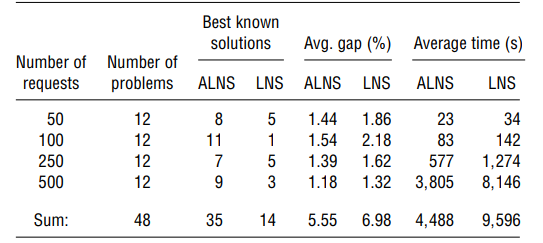
\includegraphics[scale=.6]{figures/Thuy_table6}
    \end{center}
  \textit{Ghi Chú: Chú thích của bảng được hiểu như Bảng 5. Hàng cuối cùng tính tổng mỗi cột. Lưu ý rằng quy mô của các vấn đề trong bảng này được đưa ra dưới dạng số lượng yêu cầu chứ không phải số lượng vị trí.}
    \end{figure}
\end{center}

Chúng tôi quan sát các xu hướng tương tự như trong Bảng 5; ALNS vẫn vượt trội hơn so với LNS, nhưng người ta nhận thấy rằng khoảng cách về chất lượng giải pháp giữa hai phương pháp đối với tập các điều chỉnh này nhỏ hơn trong khi sự khác biệt về thời gian chạy lớn hơn so với kết quả trên các trường hợp của Li Và Lim (2001). Người ta cũng nhận thấy rằng việc giải các trường hợp nhỏ của lớp bài toán này dường như khó hơn so với các trường hợp Li Và Lim.

Bảng 8 tóm tắt các đặc tính của vấn đề ảnh hưởng như thế nào đến chất lượng giải pháp trung bình. Những kết quả này cho thấy rằng các vấn đề phân cụm là khó giải quyết nhất, trong khi các trường hợp phân bố đồng đều là dễ nhất. Kết quả cũng chỉ ra rằng các yêu cầu đặc biệt khiến vấn đề khó giải quyết hơn một chút. Các thử nghiệm về loại tuyến đường so sánh tình huống mà các tuyến đường bắt đầu và kết thúc tại cùng một vị trí (tình huống điển hình được xem xét trong tài liệu) với tình huống mỗi tuyến đường bắt đầu và kết thúc ở các vị trí khác nhau. Ở đây, chúng tôi hy vọng trường hợp cuối cùng sẽ dễ giải quyết hơn, vì chúng tôi có các tuyến đường mà vị trí bắt đầu và kết thúc khác nhau, từ đó sẽ có được thông tin về khu vực mà tuyến đường có nhiều khả năng sẽ đi qua nhất. Các kết quả trong Bảng 8 xác nhận những kỳ vọng này.
Ngoài việc điều tra câu hỏi về cách các đặc tính của mô hình ảnh hưởng đến chất lượng giải pháp trung bình thu được từ heuristics, chúng tôi cũng muốn biết liệu sự hiện diện của một số đặc tính có thể khiến LNS hoạt động tốt hơn ALNS hay không. Đối với các đặc tính được xem xét, câu trả lời là tiêu cực.

\section{So sánh với các phương pháp heuristics hiện có}
Phần này so sánh các phương pháp ALNS heuristics với các phương pháp heuristics hiện có cho PDPTW. Việc so sánh được thực hiện bằng cách sử dụng các trường hợp điểm chuẩn do Li và Lim (2001) đề xuất, cũng được sử dụng trong phần 4.4.2. Khi các vấn đề PDPTW đã được giải quyết trong tài liệu, mục tiêu chính là giảm thiểu số lượng phương tiện được sử dụng, trong khi mục tiêu phụ là giảm thiểu quãng đường di chuyển. Với mục đích này, chúng tôi sử dụng thuật toán giảm thiểu phương tiện được mô tả trong Phần 3.7. ALNS heuristic được áp dụng 10 lần cho mỗi trường hợp có 200 vị trí trở xuống và 5 lần cho mỗi trường hợp có hơn 200 vị trí. Các thử nghiệm được tóm tắt trong Bảng 7, 9 và 10. Cần lưu ý rằng cần phải giảm tham số w và tăng tham số c khi các trường hợp có 1,000 vị trí được giải quyết để có được chất lượng giải pháp hợp lý. Ngoài ra, các tham số được cài đặt giống nhau đã được sử dụng cho tất cả các trường hợp.

\begin{center}
    \begin{figure}[htp]
    \caption{So sánh ALNS Heuristic và Heuristics hiện có}        
    \begin{center}
     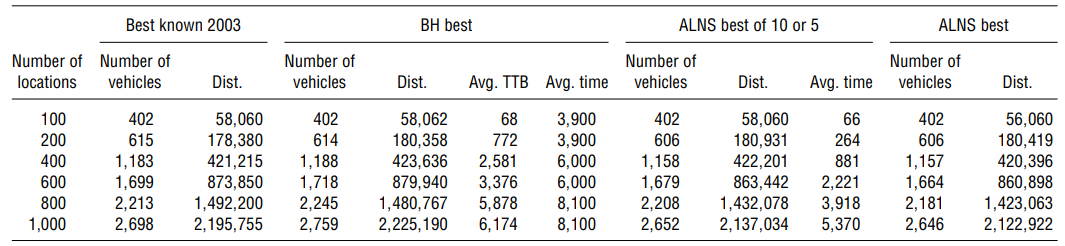
\includegraphics[scale=.5]{figures/Thuy_table7}
    \end{center}
  \textit{Ghi Chú: Mỗi hàng trong bảng tương ứng với một tập hợp các vấn đề có cùng số vị trí. Mỗi tập hợp vấn đề này chứa từ 56 đến 60 trường hợp (xem Bảng 9). Cột đầu tiên cho biết số lượng vị trí trong mỗi vấn đề; hai cột tiếp theo đưa ra tổng số phương tiện được sử dụng và tổng quãng đường di chuyển trong các giải pháp nổi tiếng nhất trước đây như được liệt kê trên trang web SINTEF vào mùa hè năm 2003. Bốn cột tiếp theo hiển thị thông tin về các giải pháp có được từ phương pháp heuristic của Bent và Van Hentenryck (2003a). Hai cột Avg.TTB và Avg.Time lần lượt hiển thị thời gian trung bình cần thiết để đạt được giải pháp tốt nhất và thời gian trung bình dành cho từng trường hợp. Cả hai cột đều báo cáo thời gian cần thiết để thực hiện một thử nghiệm trên một phiên bản. Ba cột tiếp theo báo cáo các giải pháp thu được trong thử nghiệm với phương pháp ALNS heuristic trong đó phương pháp heuristic được áp dụng 5 hoặc 10 lần cho mỗi vấn đề. Hai cột cuối cùng báo cáo các giải pháp tốt nhất thu được trong một số thử nghiệm với ALNS heuristic của chúng tôi và với các cài đặt tham số khác nhau. Lưu ý rằng Bent và Van Hentenryck trong một số trường hợp đã tìm thấy kết quả tốt hơn một chút so với báo cáo trên trang web SINTEF năm 2003. Đây là lý do tại sao số lượng phương tiện được sử dụng bởi BH heuristic cho các bài toán 200 vị trí lại nhỏ hơn so với bài toán được biết đến nhiều nhất.}
    \end{figure}
\end{center}


\begin{center}
    \begin{figure}[htp]
    \caption{Tóm tắt ảnh hưởng của một số đặc tính của vấn đề đối với phương pháp heuristics}        
    \begin{center}
     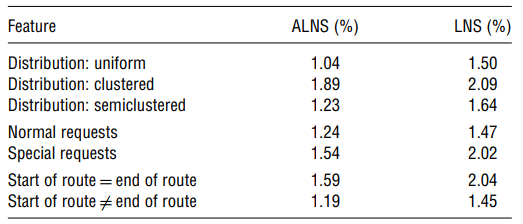
\includegraphics[scale=.5]{figures/Thuy_table8}
    \end{center}
    \end{figure}
\end{center}


\begin{center}
    \begin{figure}[htp]
    \caption{So sánh với các giải pháp được biết đến nhiều nhất trước đây}        
    \begin{center}
     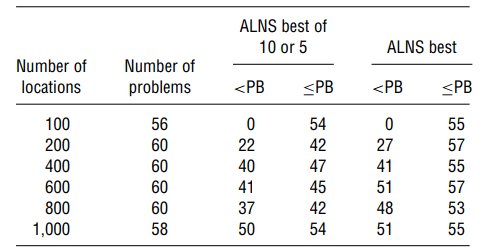
\includegraphics[scale=.5]{figures/Thuy_table9}
    \end{center}
  \textit{Ghi Chú: Bảng được nhóm theo quy mô vấn đề. Cột đầu tiên hiển thị quy mô vấn đề; cột tiếp theo hiển thị số vấn đề có kích thước đó. Hai cột tiếp theo cung cấp thông tin bổ sung về thử nghiệm trong đó phương pháp ALNS heuristics được áp dụng 5 hoặc 10 lần cho mỗi trường hợp. Các cột < PB báo cáo số lần giải pháp tốt nhất được tìm ra bởi ALNS heuristic tốt hơn hoàn toàn so với giải pháp tốt nhất đã biết trước đó. Các cột ≤ PB cho biết giải pháp tốt nhất do ALNS tìm thấy ít nhất tốt bằng giải pháp tốt nhất đã biết trước đây. Hai cột cuối cùng hiển thị thông tin về các giải pháp tốt nhất thu được trong quá trình thử nghiệm với các cài đặt tham số khác nhau.}
    \end{figure}
\end{center}


\begin{center}
    \begin{figure}[htp]
    \caption{Hiệu suất trung bình của ALNS heuristics}        
    \begin{center}
     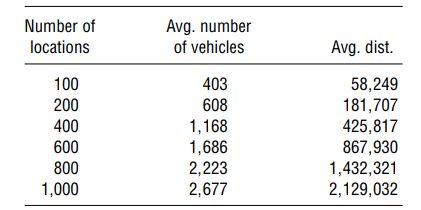
\includegraphics[scale=.7]{figures/Thuy_table10}
    \end{center}
  \textit{Ghi Chú: Các giải pháp tốt nhất được báo cáo trong Bảng 7 và 9 tất nhiên không thu được trong tất cả các thí nghiệm. Bảng này cho biết số lượng phương tiện trung bình và quãng đường trung bình đã đi. Những con số này có thể được so sánh với những con số trong Bảng 7.}
    \end{figure}
\end{center}

Trong tài liệu, bốn heuristics đã được áp dụng cho các bài toán điểm chuẩn: Heuristic của Li và Lim (2001), Heuristic của Bent và Van Henten-ryck (2003a), và hai heuristic thương mại: heuristic do SINTEF phát triển và heuristic do TetraSoft A/S phát triển. Các kết quả chi tiết cho heuristic cuối cùng không có sẵn, nhưng một số kết quả thu được bằng cách sử dụng các heuristic này có thể được tìm thấy trên một trang web do SINTEF ntef khai thác (http://www.sintef.no/static/am/opti/projects/top /vrp/ benchmarks.html).

Phương pháp heuristic thu được chất lượng giải pháp tổng thể tốt nhất cho đến nay có lẽ là phương pháp của be Bent và Van Henten-ryck (2003a) (được rút gọn thành phương pháp phỏng đoán BH ở phần sau), do đó phương pháp phỏng đoán ALNS được so sánh với phương pháp phỏng đoán này trong Bảng 7. Các kết quả đầy đủ từ phương pháp BH heuristic có thể được tìm thấy trong Bent và Van Henten-ryck (2003b). Các kết quả của phương pháp BH heuristic là kết quả tốt nhất thu được trong số 10 thử nghiệm (mặc dù đối với trường hợp 100 vị trí, chỉ có 5 thử nghiệm được thực hiện). Cột Avg. TTB hiển thị thời gian trung bình cần thiết để chẩn đoán BH có được giải pháp tốt nhất. Đối với ALNS heuristic, chúng tôi chỉ liệt kê tổng thời gian đã sử dụng vì heuristic này - do thành phần ủ mô phỏng của nó - thường tìm ra giải pháp tốt nhất vào cuối quá trình tìm kiếm. Thử nghiệm BH đã được thử nghiệm trên bộ xử lý Athlon 1.2 GHz và do đó, thời gian chạy của hai thử nghiệm phải tương đương nhau (chúng tôi tin rằng bộ xử lý Athlon chậm hơn nhiều nhất là 20\% so với máy tính của chúng tôi). Các kết quả cho thấy rằng về tổng thể, ALNS heuristic chiếm ưu thế hơn BH heuristic, đặc biệt là khi kích thước của vấn đề tăng lên. Rõ ràng là phương pháp ALNS heuristic có thể cải thiện đáng kể các giải pháp đã biết trước đây và dù khá đơn giản nhưng thuật toán giảm số lượng phương tiện cũng hoạt động rất tốt. Hai cột cuối cùng trong bảng 7 tóm tắt các kết quả tốt nhất thu được bằng cách sử dụng một số thử nghiệm với các cài đặt tham số khác nhau, cho thấy rằng các kết quả thu được bằng ALNS thực sự có thể được cải thiện hơn nữa.

Bảng 9 so sánh các kết quả thu được từ ALNS với các giải pháp được biết đến nhiều nhất từ tài liệu. Có thể thấy rằng ALNS cải thiện hơn một nửa số giải pháp và đạt được giải pháp ít nhất cũng tốt bằng giải pháp tốt nhất đã biết trước đây cho 80\% vấn đề.

Hai bảng nói trên chỉ xử lý các giải pháp tốt nhất được tìm thấy bởi ALNS heuristic. Bảng 10 cho thấy chất lượng trung bình của giải pháp thu được bằng heuristic. Những con số này có thể được so sánh với những con số trong Bảng 7. Điều đáng chú ý là giải pháp trung bình đôi khi có khoảng cách thấp hơn so với giải pháp “tốt nhất trong số 10 hoặc 5” trong Bảng 7; Đây chính là trường hợp ở hàng cuối cùng. Điều này là có thể vì heuristic tìm ra các giải pháp sử dụng nhiều hơn số lượng phương tiện tối thiểu và điều này thường tạo ra các giải pháp với khoảng cách ngắn hơn.
Nhìn chung, có thể kết luận rằng ALNS heuristic phải được coi là một heuristic tiên tiến nhất cho PDPTW. Chi phí của các giải pháp tốt nhất được xác định trong các thí nghiệm được liệt kê trong Bảng 11 đến 16.

\begin{center}
    \begin{figure}[htp]
    \caption{Kết quả tốt nhất, 100 địa điểm}        
    \begin{center}
     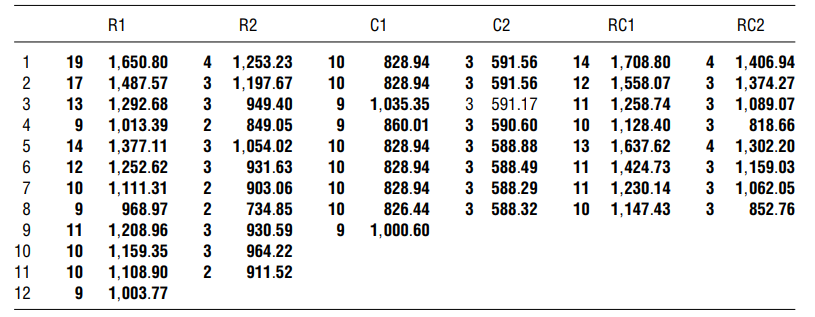
\includegraphics[scale=.5]{figures/Thuy_table11}
    \end{center}
  \textit{Ghi Chú: Các trường hợp điểm chuẩn của Li và Lim (2001) được chia thành sáu bộ: R1, R2, C1, C2, RC1 và RC2. Mỗi cột chính tương ứng với một trong những bộ này; cột bên trái đưa ra số vấn đề. Đối với mỗi trường hợp vấn đề, chúng tôi báo cáo số lượng phương tiện và quãng đường di chuyển trong giải pháp tốt nhất thu được trong quá trình thử nghiệm. Số in đậm chỉ ra các giải pháp được biết đến nhiều nhất.}
    \end{figure}
\end{center}


\begin{center}
    \begin{figure}[htp]
    \caption{Kết quả tốt nhất, 200 địa điểm}        
    \begin{center}
     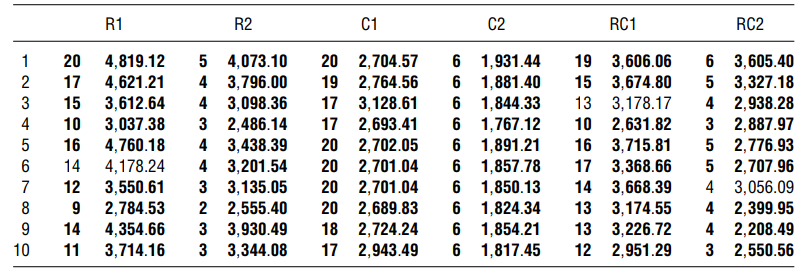
\includegraphics[scale=.5]{figures/Thuy_table12}
    \end{center} 
    \end{figure}
\end{center}

\begin{center}
    \begin{figure}[htp]
    \caption{Kết quả tốt nhất, 400 địa điểm}        
    \begin{center}
     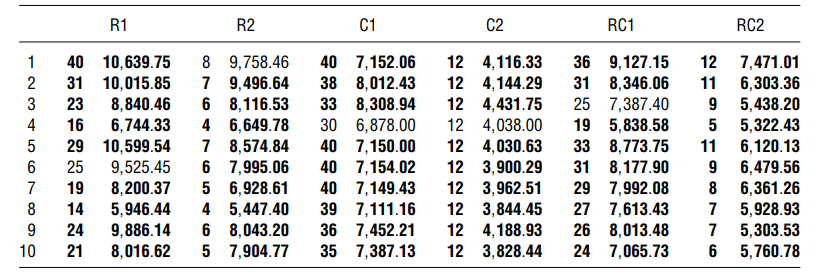
\includegraphics[scale=.5]{figures/Thuy_table13}
    \end{center}
    \end{figure}
\end{center}

\begin{center}
    \begin{figure}[htp]
    \caption{Kết quả tốt nhất, 600 địa điểm}        
    \begin{center}
     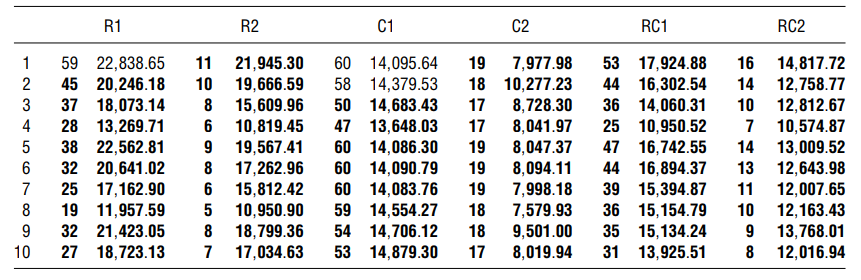
\includegraphics[scale=.5]{figures/Thuy_table14}
    \end{center}
    \end{figure}
\end{center}

\begin{center}
    \begin{figure}[htp]
    \caption{Kết quả tốt nhất, 800 địa điểm}        
    \begin{center}
     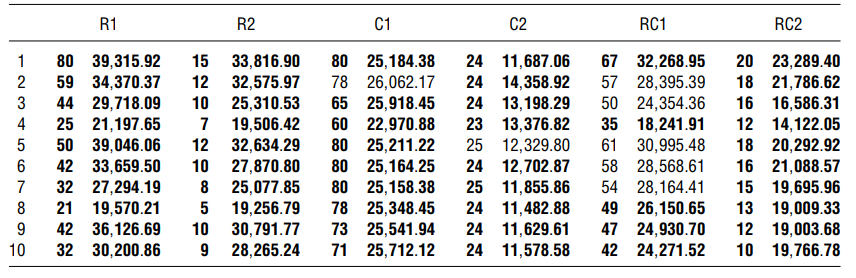
\includegraphics[scale=.5]{figures/Thuy_table15}
    \end{center}
    \end{figure}
\end{center}

\begin{center}
    \begin{figure}[htp]
    \caption{Kết quả tốt nhất, 1,000 địa điểm}        
    \begin{center}
     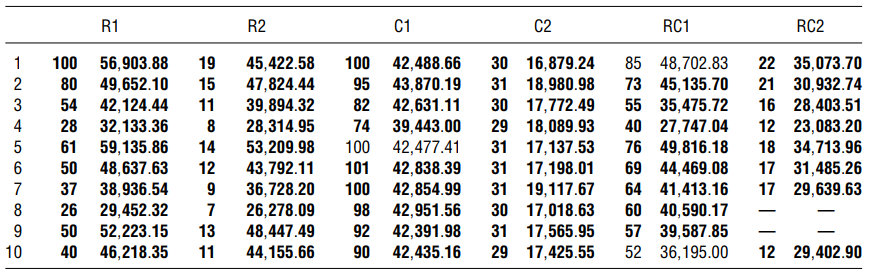
\includegraphics[scale=.5]{figures/Thuy_table16}
    \end{center}
    \end{figure}
\end{center}


\subsection{Kết luận các tính toán thí nghiệm}
Trong phần 4.4, chúng tôi đã nêu ba mục tiêu cho các tính toán thí nghiệm. Các thí nghiệm đã hoàn thành các mục tiêu này khi chúng tôi thấy rằng: (1) phương pháp LNS heuristic thích hợp kết hợp một số phương pháp loại bỏ và construction heuristic hiển thị hiệu suất vượt trội so với phương pháp LNS heuristic đơn giản chỉ sử dụng một phương pháp heuristic thêm và một phương pháp heuristic xóa; (2) một số đặc điểm của vấn đề ảnh hưởng đến hiệu suất của phương pháp LNS heuristic, nhưng chúng tôi không thấy rằng bất kỳ đặc điểm nào có thể làm cho phương pháp LNS heuristic hoạt động tốt hơn phương pháp ALNS heuristic; (3) phương pháp LNS heuristic thực sự có thể tìm thấy các giải pháp chất lượng tốt trong một khoảng thời gian hợp lý và heuristic vượt trội so với các heuristic được đề xuất trước đó.

Các thí nghiệm cũng minh họa tầm quan trọng của việc thử nghiệm heuristic trên các tập hợp lớn các vấn đề, bởi vì sự khác biệt giữa LNS và ALNS chỉ thực sự trở nên rõ ràng khi chúng ta xem xét các trường hợp lớn. Lưu ý rằng các vấn đề cần giải quyết trong thế giới thực thường có kích thước tương đương hoặc lớn hơn các vấn đề lớn nhất được giải quyết trong bài báo này.

Cuối cùng, các tính toán thí nghiệm được thực hiện trong phần 4.3.3 chỉ ra rằng phương pháp LNS heuristic đơn giản dường như nhạy cảm với các lựa chọn của phương pháp heuristic xóa, hơn là với các lựa chọn của phương pháp heuristic thêm. Sẽ rất thú vị nếu điều này nói chung đúng cho các vấn đề khác.
